\begin{part}{Quantifiers and Set-Like Objects}
    So, we introduced you to modal logic, which gives us the ability to discuss possibility and necessity. Now, we are ready to take that a bit further, and discuss how 
    
    to sets as logic object, and we have discussed how quantifiers 
    
    Discuss how sets have the feel of ``Boolean membership'', and could be described as the universe with (T, a), (F, b)
    \begin{chapter}{Unnamed}
        \begin{section}{Sets Can Contain Sets}
            There is nothing stopping a set from containing another set, just as if there is nothing to stop a bag from holding another bag, empty or not. Furthermore, a bag, containing an empty bag, has contents, and is therefore not interchangeable with each other (despite that the empty bag inside is):
            
            $$
                \{ \{\} \} \neq \{ \}
            $$
            
            We can use make use of this too. For instance, we can define our Boolean Domain as:
            
            \begin{gather*}
                F = \{ \} \\
                T = \{ \{ \} \} \\
                \mathbb{B} = \{F, T\} = \{\{\}, \{ \{ \} \} \}
            \end{gather*}
            
            \begin{samepage}
                This definition means that, we have a set of 2 items: the first item is an empty set, and the second item is a set containing an empty set:
                \begin{figure}[ht]
                    \centering
                    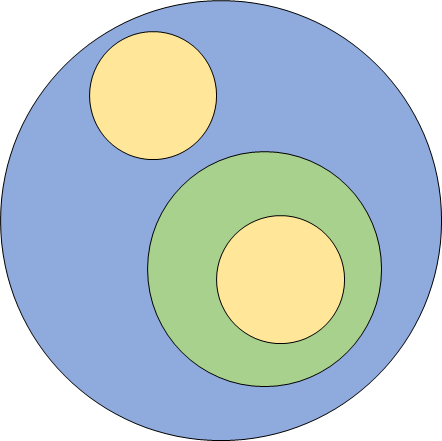
\includegraphics[scale=0.5]{Sets/BooleansAsSets}
                    \caption{Boolean Domain Defined as Sets.}
                    \label{fig:BooleanDomainDefinedAsSets}
                \end{figure}
            \end{samepage}
            
            We could keep nesting sets in sets in sets. This would give us a way to demonstrate the Natural Numbers. Let's do a few examples:
            \begin{gather*}
                0 = \{ \} \\
                1 = 0 \cup \{ 0 \} = \{ \{ \} \} \\
                2 = 1 \cup \{ 1 \} = \{ \{ \}, \{ \{ \} \} \}
            \end{gather*}
        \end{section}
        \begin{section}{Additional Set Options}
            \begin{subsection}{Set Comprehensions}
                We have discussed building up sets according to their elements. However, often, we want to define a subset according to some filtering predicate. We call this set comprehension, and it looks like this:
                
                $$
                    \{ x \in \mathbb{Z} : x \leq 3 \}
                $$
                
                Which is the list of all natural numbers below 3. This is the same as:
                $$
                    \{ x \in \mathbb{Z} : x \leq 3 \} = \{0, 1, 2, 3\}
                $$
            \end{subsection}
        
            \begin{subsection}{Cardinality}
                Oftentimes, we are also interested in how many items are in a set. For instance, we may have a set A:
                $$
                    A \defeq \{\texttt{red}, \texttt{green}, \texttt{blue}\}
                $$
                So, we define an operation, called the \textbf{cardinality} of the set, with the purpose of telling us how many elements there are. In programming, you may find that this operation as:
                
                \begin{verbatim}
                    cardinality = set.Length;
                \end{verbatim}
                \begin{verbatim}
                    cardinality = set.Count;
                \end{verbatim}
                
                And, symbolically, we encode this as $|A|$, which is 2 bars surrounding the set, and we find that when we compute this, we get:
                $$
                    |A| \vdash 3
                $$
                
                The cardinality can seem supplemental and not useful for working with sets, but it can demonstrate counting for us.
                
                If we had a way to add a new element to a set, and know that element wasn't already a member of the set, then we know that we'd increase the cardinality by 1. This property can help us prove properties of natural numbers, and we will be doing this, but probably using types instead of sets.
            \end{subsection}
            \begin{subsection}{Cartesian Product}
                Here is where things get interesting. It may not seem like it at first, because we can intuitively see so many benefits to unions, intersections, and things like that, operations like the Cartesian Product seem weird and unintuitive at first, but given that the name Cartesian is from René Descartés, we can begin to consider that this has something to do with geometry.
                
                So, the Cartesian Product creates ordered pairs from sets. Now, let's talk about this word ``order'' a bit before we continue. In this case here, it means that we could index the items by saying, ``this item occurs 1st in the collection, and this next item occurs 2nd''.
                
                \todo{Move the curly bracket discussion up}
                As you'll remember, sets are unordered. There is no way to index them. Sets also use curly brackets ( $\{ \}$ ). When talking about collections that can be fully indexed (all items can be put in order), we will use parentheses.
                
                So, the cartesian product takes elements from a set A, and elements from a set B, and gives us a pair of all possible combinations of the two:
                
                \begin{table}[ht]
                    \centering
                    \begin{tabular}{|c|c|c|c|c|}
                        \hline
                        \multicolumn{2}{|c|}{\multirow{2}{*}{$A \times B$}} & \multicolumn{3}{c|}{B} \\ \cline{3-5} 
                        \multicolumn{2}{|c|}{} & red & green & blue \\ \hline
                        \multirow{2}{*}{A} & square & (square, red) & (square, green) & (square, blue) \\ \cline{2-5} 
                         & triangle & (triangle, red) & (triangle, green) & (triangle, blue) \\ \hline
                        \end{tabular}
                    \caption{Cartesian Product in Operator Table.}
                    \label{CartesianProductOperatorTable}
                \end{table}
                
                If you remember how multiplication can be used to count the number of tiles horizontally and vertically, you will notice that the number of elements in A is 2, and the number of elements in B is 3; therefore, the number of elements in $A\times B$ is $2 \times 3 = 6$.
                
                If we add another shape to $A$, then there will be 3 more elements in the cartesian product, giving us $3 \times 3 = 9$. If instead, we had added an additional color to B, we would have to add 2 more elements to the cartesian product, which would give us $2 \times 4 = 8$. Therefore, you should be able to see why the word ``product'', which seems to imply multiplication, is used to describe this operation:
                
                \begin{equation}
                    |A \times B| = |A| \times |B|
                \end{equation}
                
                We still haven't defined natural numbers yet, but using the assumption that you can already count with them, you'll see that the if we create the cartesian product of two sets, then we get the cardinality (count), this is equivalent to the cardinality of each set multiplied together.
                
                Now, it's important to stop you here and ask, is this cartesian product commutative? Is it associative?
                
                This is difficult to discuss, because it depends on context. Remember before when we talked about isomorphisms. If we are interested only in whether or not we can match one element to another, then it is commutative. However, we may very well be working in a context where an ordered pair can contain a primitive element and another ordered pair:
                $$
                    (a, (b, c)) \neq  (a, b, c) \neq ((a, b), c)
                $$
                All 3 of these may be the same, or different. When we consider them different, we still usually discuss some way to convert from one to another. Remember before that, if we can convert, then there is an isomorphism (equal usage), and if there is an isomophism, then there is an equality that can be created by that.
                
                However, we will \textbf{NOT} immediately be working with the context that these are equal.
                
                Additionally, we'll explain here that the introduction of the Cartesian Product before the Natural Numbers, in this case, was only done to demonstrate why this is called a ``Product'', and link it to your intuitions of multiplication.
                
                We have, however, introduced the Boolean Domain, and for a moment, if we are allowed to use $\{0, 1\}$ from the Boolean Domain, then it's enough for us to demonstrate one way to generate an ordered pair from a set.
                
                Imagine sets A of shapes, and B of colors before. We need to create a single element of the cartesian product. For this, we will talk about the element (square,red).
                
                For this, we use the Natural Numbers as part of our set:
                $$
                    (\textsc{square}, \textsc{red} ) = \{\{0, \textsc{square}\}, \{1, \textsc{red}\}\}
                $$
                
                It's another set containing sets.
                
                This means that, even if we were to swap square and red, square comes before red, because 0 goes with it. Likewise, 1 goes with red.
                
                This means that, in general, for any a and b, we can create an ordered pair from it:
                
                $$
                    (a, b) = \{\{0, a\}, \{1, b\}\}
                $$
                
                This leaves us with:
                \begin{enumerate}
                    \item Ordered pairs, represented as $(a, b)$
                    \item Cartesian Product of 2 sets, represented as $A \times B$, and giving us elements that are ordered pairs, defined as $\{ \forall a\in A : \forall b \in B : (a, b) \}$
                \end{enumerate}
                
                However, we can also do some of the same tricks we did before when we defined the Boolean Domain and the Natural Numbers.
                
                $$
                    (a, b) = \{ \{a\}, \{a, b\} \}
                    (b, a) = \{ \{b\}, \{a, b\} \}
                $$
                
                Now, it took years to discover this construction, and we can thank  Kazimierz Kuratowski for this construction. The beauty is that if we take the intersection of the inner sets of $(a, b)$, we get $\{ \{ a \} \}$, and the intersection of the inner sets of $(b, a)$, gives us $\{ \{ b \} \}$.
                
                If we have an ordered pair that looks like $(a, a)$, such that the elements are actually a pair of the same thing, then we end up with:
                
                $$
                    (a, a) = \{ \{ a \}, \{a, a \} \} = \{ \{ a \}, \{ a \} \} = \{ \{ a \} \}
                $$
                
                We can remove these from the curly braces, and we can get the second element too, but we will need to go a little farther for that.
            \end{subsection}
            \begin{subsection}{Disjoint Union}
                The Disjoint Union has some similarities to the union. The idea is to combine the elements from two sets. If two sets have no elements in common, they are called disjoint, and have a Venn diagram like the following:
                \todo{Venn diagram of disjoint sets}
                
                The disjoint union attempts to put sets together, and include a tracking marker that tells you what set they came from. It is defined as:
                $$
                    A \sqcup B = \{A \times \{0\}\} \cup \{B \times \{1\}\}
                $$
                
                Let's use some new sets for our example:
                $$
                    A = \{\textsc{red}, \textsc{green}, \textsc{blue}\}
                $$
                
                $$
                    B = \{\textsc{yellow}, \textsc{green}, \textsc{cyan}\}
                $$
                
                Using our color sets, we would end up with a set that looks like the following:
                $$
                    A \sqcup B = \{ (\textsc{red}, 0), (\textsc{green}, 0), (\textsc{blue}, 0), (\textsc{yellow}, 1), (\textsc{green}, 1), (\textsc{blue}, 1)\}
                $$
                
                You will notice there that green occurs twice, but the marker tells it which set green came from, so one green came from the first set, and one green came from the second. You'll also notice that the number of elements that are in the disjoint union are the number of elements in set A plus the elements in set B:
                
                $$
                    |A \sqcup B| = |A| + |B|  
                $$
            \end{subsection}
            \begin{subsection}{Big Operators}
                Now that we have all of that hashed out, and we have talked about sets containing sets, let's talk about taking the intersection of a bunch of sets... contained in a bigger set:
                
                $$
                    \bigcap \{ \{ \textsc{red} \}, \{ \textsc{green}, \textsc{red} \}, \{\textsc{red}, \textsc{blue}\} \}=
                    \{ \textsc{red} \} \cup \{ \textsc{green}, \textsc{red} \} \cup \{\textsc{red}, \textsc{blue}\} = \{ \textsc{red} \}
                $$
                
                Some important things happen here....
                \begin{enumerate}
                    \item We must know that the set we are working on, \textbf{contains only sets}. So far, Booleans, Natural Numbers, Cartesian Products and Disjoint Unions have been shown to give us sets of sets. However, we do not necessarily know this in general (and for that, we will need to get into types).
                    
                    \item It gives us a set from a set of sets, seeming to remove a layer. Because we remove a layer, we can also take a single element out of curly brackets, assuming we know that it's a set (if it's not, we can handle this specific case below):
                    $$
                        \bigcup {a} = a
                    $$
                    
                    \item It lets us do this for an arbitrary number of contained sets.
                \end{enumerate}
                
                Using this, we can go back to our definition of Cartesian Product and attempt to obtain the 2 elements from our set:
                
                $$
                    \bigcup\bigcap \{ \{ a \}, \{ a, b \} \} = \bigcup \{ a \} = a
                $$
                
                And we can get the second element by testing if $\bigcup S \setminus \bigcap S = \{ \}$. If it is, it's the same element (i.e. $(a, a)$). If it's not, then the result is $\bigcup (\bigcup S \setminus \bigcap S)$
                
                In the case that we have $(a, a)$ then we get:
                
                $$
                    \bigcup \{ \{ a \} \} \setminus \bigcap \{ \{ a \} \} = \{ \}
                $$
                
                In the case that we have $(a, b)$, then we get:
                \begin{gather*}
                    \bigcup \left(\bigcup \{ \{ a \}, \{ a, b \} \} \setminus \bigcap \{ \{ a \}, \{ a, b \} \} \right) \\
                    \bigcup \left(\{a, b\} \setminus \{ a \}\right) \\
                    \bigcup \{ b \} = b
                \end{gather*}
                
                
            \end{subsection}
            
            \begin{subsection}{Multiplication and Addition}
                Think really hard about this now. We have defined Natural Numbers earlier, and we have talked about disjoint union, which works like addition of sets (at least through cardinality).
                
                What then, is 0 + 1, according to our definition?
                
            \end{subsection}
            
        \end{section}
        \begin{section}{Barber's Paradoxes and the Set}
            A physical bag is a close analogy to what's called a multiset (a set that allows duplicates), but one part of the analogy that I'd like to bring to the set conversation is that a physical bag cannot contain itself without some extreme mental gymnastics (i.e. changing the meaning of the word ``contain'').
            
            Likewise, a set cannot contain itself. Mathematically, it seems as if this was arbitrary, but let's consider a particular paradox for a moment:
            \begin{quote}
                Imagine a barber that only shaves those that do not shave themselves. Does this barber shave himself?
            \end{quote}
            
            If the barber shaves himself, then there is at least one person he shaves that shaves himself (i.e. himself). If he does not shave himself, then there is at least one person that he doesn't shave that doesn't shave himself (i.e. himself).
            
            Likewise, we can define a set that contains all sets that do not contain themselves. Using the barber analogy, that set results in a logical inconsistency that cannot be resolved. Therefore, we want to control the construction of a set, and some of the axioms are used to eliminate such an inconsistent case.
        \end{section}
    \end{chapter}
    
    \begin{chapter}{Binary Relations}
        \begin{definition}
            We define a binary relation (R) between 2 sets, A and B, to be a subset of the Cartesian Product of the 2 sets ($R \in A \times B$).
        \end{definition}
        
        This definition allows us to say that an element $a_1$ relates to an element $b_2$ and so forth. We can draw this using a digraph:
        
        \begin{figure}
            \centering
            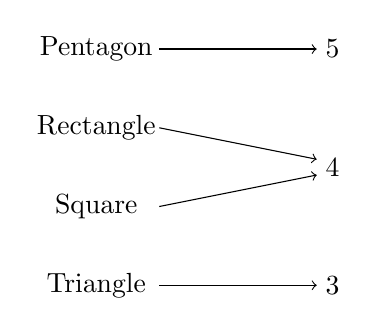
\begin{tikzpicture}
                \draw[align=right] (0, 0) node {Triangle};
                \draw[align=right] (0, 1) node {Square};
                \draw[align=right] (0, 2) node {Rectangle};
                \draw[align=right] (0, 3) node {Pentagon};
                
                \draw (3, 0.0) node {3};
                \draw (3, 1.5) node {4};
                \draw (3, 3.0) node {5};
                
                \draw [->] (0.8, 0) -- (2.8, 0.0);
                \draw [->] (0.8, 1) -- (2.8, 1.4);
                \draw [->] (0.8, 2) -- (2.8, 1.6);
                \draw [->] (0.8, 3) -- (2.8, 3.0);
            \end{tikzpicture}
            \caption{Digraph Relationship Between Polygons and the Number of Sides.}
            \label{fig:RelationshipBetweenPolygonsAndSides}
        \end{figure}
        
        Giving our relation between A and B the symbol $A \sim B$, we can also put them in a Cayley Predicate Table:
        
        \begin{table}[ht]
            \centering
            \begin{tabular}{|c|c|c|c|c|}
                \hline
                \multicolumn{2}{|c|}{\multirow{2}{*}{$A \sim B$}} & \multicolumn{3}{c|}{B} \\ \cline{3-5} 
                \multicolumn{2}{|c|}{} & 5 & 4 & 3 \\ \hline
                \multirow{4}{*}{A} & Pentagon & \cmark & \xmark & \xmark \\ \cline{2-5} 
                 & Rectangle & \xmark & \cmark & \xmark \\ \cline{2-5} 
                 & Square & \xmark & \cmark & \xmark \\ \cline{2-5} 
                 & Triangle & \xmark & \xmark & \cmark \\ \hline
            \end{tabular}
            \caption{Cayley Predicate Table of Relation Between Polynomials and Sides.}
            \label{tab:CayleyPredicateTableRelationPolynomialsSides}
        \end{table}
        
        Note from both table and digraph that $A \sim B \neq B \sim A$. In other words, it is not commutative, but we WILL discuss associativity.
        
        Discuss composition through ``matrix multiplication''. Discuss different symbolic ways to represent relations.
        
        You can notice that by looking at the Cayley Predicate Table that the checkmark (\cmark) is found exactly once per row of A. This is equivalent to saying that, on the diagraph, that there is exactly one arrow coming from each object of the shapes set.
        
        \begin{definition}
            A left-unique 
        \end{definition}
        
        A function in pure mathematics is not a function in computer science, despite that computer science is an offshoot of mathematcics (around the foundations of mathematics). The context of the word function changes in computer science to include side-effects, let's start with state and then go to sessions.
    
        Unary relations are set comprehensions
        \begin{section}{Function-Like Relations}
        \end{section}
        
        \begin{section}{Order-like Relations}
        
        \end{section}
        
        \begin{section}{Equivalence Relations}
        \end{section}
    \end{chapter}
    \begin{chapter}{Counting and Combinatorics}
        \begin{section}{adsf}
            \begin{subsection}{Relationships on the Boolean Algebra}
                \begin{align*}
                    |A \cap B| \leq |A| \quad  \textrm{and} \quad  |A \cap B| \leq |B|
                \end{align*}
                
                This is directly related to the fact that:
                \begin{align*}
                    X \subseteq Y \implies |X| \leq |Y|
                \end{align*}
                
                And this connection between these two, as important as it is, will be more thoroughly described later.
            \end{subsection}
            \begin{subsection}{Addition and the Disjoint Union}
            $$
                |A \sqcup B| = |A| + |B|
            $$
            \end{subsection}
            \begin{subsection}{Multiplication and the Cartesian Product}
            $$
                |A \times B| = |A| \times |B|
            $$
            \end{subsection}
            \begin{subsection}{Functions and Exponentials}
            $$
                |A \to B| = |B|^{|A|}
            $$
            \end{subsection}
            \begin{subsection}{Powerset as a Function}
            $$
                |\mathcal{P}(X)| = | X \to \mathbb{B} | = 2^{|X|}
            $$
            \end{subsection}
            \begin{subsection}{Permutations}
                Number of permutations = number of total orders ($|A|! = n!$)
            \end{subsection}
        \end{section}
    \end{chapter}
    \begin{chapter}{Probability Theory as a Logic}
    \end{chapter}
\end{part}